\section{Thống kê mô tả}
\subsection*{4.1 Phân tích và phân chia số liệu}
Sau khi thực hiện bước tiền xử lí số liệu, ta đã làm sạch và điền khuyết dữ liệu, ta thực hiện thống kê mô tả bằng lệnh \texttt{summary()} ta sẽ có cái nhìn tổng quát hơn về bảng dữ liệu. Lệnh \texttt{summary()} sẽ xuất ra màn hình những giá trị như \textit{min} (giá trị nhỏ nhất), \textit{mean} (trung bình), \textit{median} (trung vị), \textit{Q1} (khoảng tứ phân vị thứ 1), \textit{Q3} (khoảng tứ phân vị thứ 3), \textit{max} (giá trị lớn nhất).
\begin{figure}[H]
    \centering
    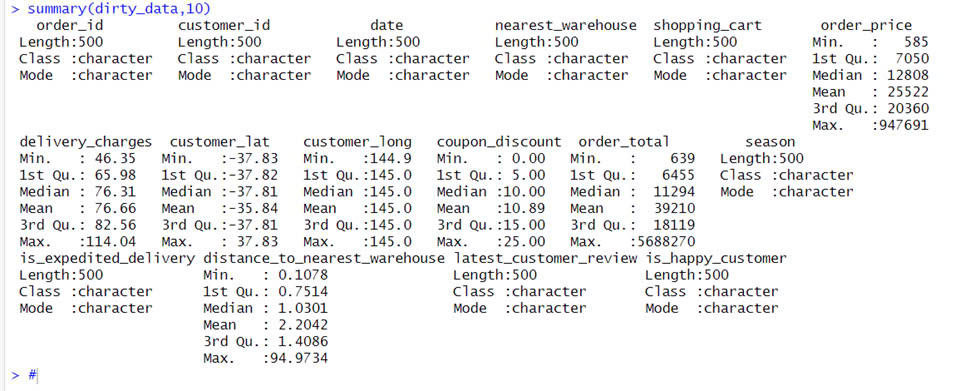
\includegraphics[width=0.9\linewidth]{graphics/bang1.jpg}
    \caption{Số liệu tổng quát}
    
\end{figure}
Sau đó ta chọn lọc những biến có thể phân tích như nearest\_warehouse, order\_price, delivery\_charges, customer\_lat, customer\_long, coupon\_discount, order\_total, season, is\_expedited\_delivery, distance\_to\_nearest\_warehouse, is\_happy\_customer. Và ta có bảng dữ liệu từ lệnh \texttt{head()}.
\begin{figure}[H]
    \centering
    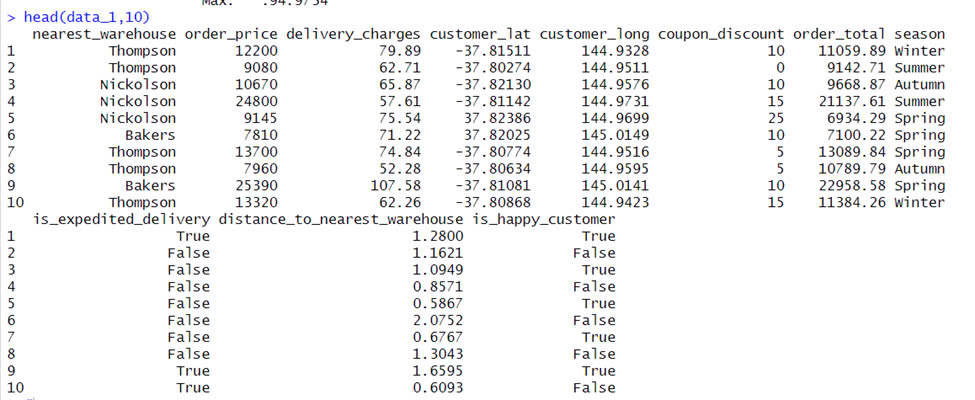
\includegraphics[width=0.9\linewidth]{graphics/bang2.jpg}
    \caption{Số liệu chọn lọc}
   
\end{figure}
            
Từ nội dung của bảng dữ liệu trên, ta tách ra thành:\\
•  Biến liên tục gồm: order\_price, delivery\_charges, customer\_lat, customer\_long, coupon\_discount, order\_total, distance\_to\_nearest\_warehouse.
 \begin{figure}[H]
    \centering
    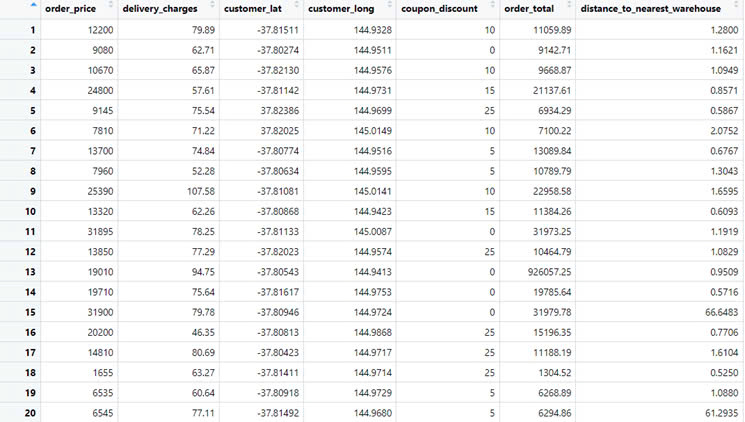
\includegraphics[width=0.9\linewidth]{graphics/bang3.jpg}
    \caption{Các biến liên tục}
   
\end{figure}
•  Biến định lượng gồm: nearest\_warehouse, season, is\_expedited\_delivery, is\_happy\_customer. Và biến định lượng được biểu diễn dưới dạng factor như sau.
\begin{figure}[H]
    \centering
    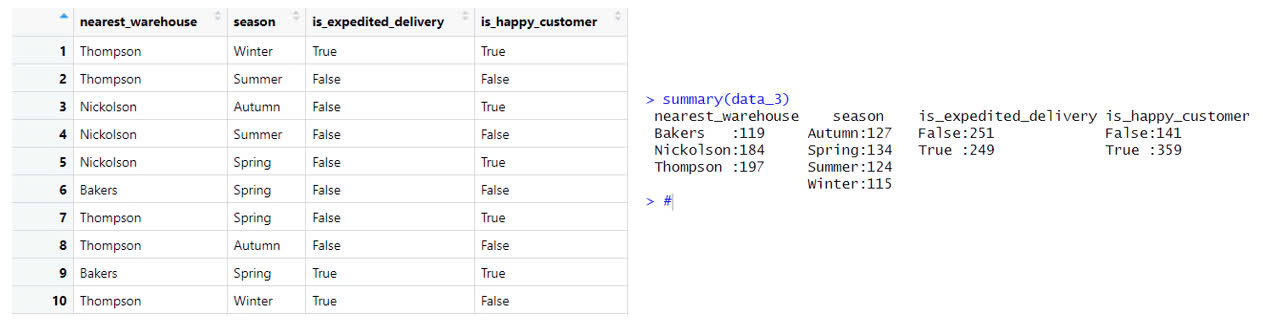
\includegraphics[width=0.9\linewidth]{graphics/bang6.jpg}
    \caption{Các biến định lượng và giá trị được biểu diễn dưới dạng factor}
   
\end{figure}
\subsection*{4.2 Phân tích biến liên tục bằng biểu đồ.}
\subsection*{\subsection*{4.2.1 Đồ thị Histogram}}
•	Vì nhóm làm phân tích các ảnh hướng đến chi phí đơn hàng nên sẽ không có customer\_lat và customer\_long. Dưới đây là một số hình ảnh của các biến order\_price, delivery\_charges, coupon\_discount, order\_total, distance\_to\_nearest\_warehouse. Khi biểu diễn bằng đồ thị Histogram

\begin{figure}[H]
    \centering
    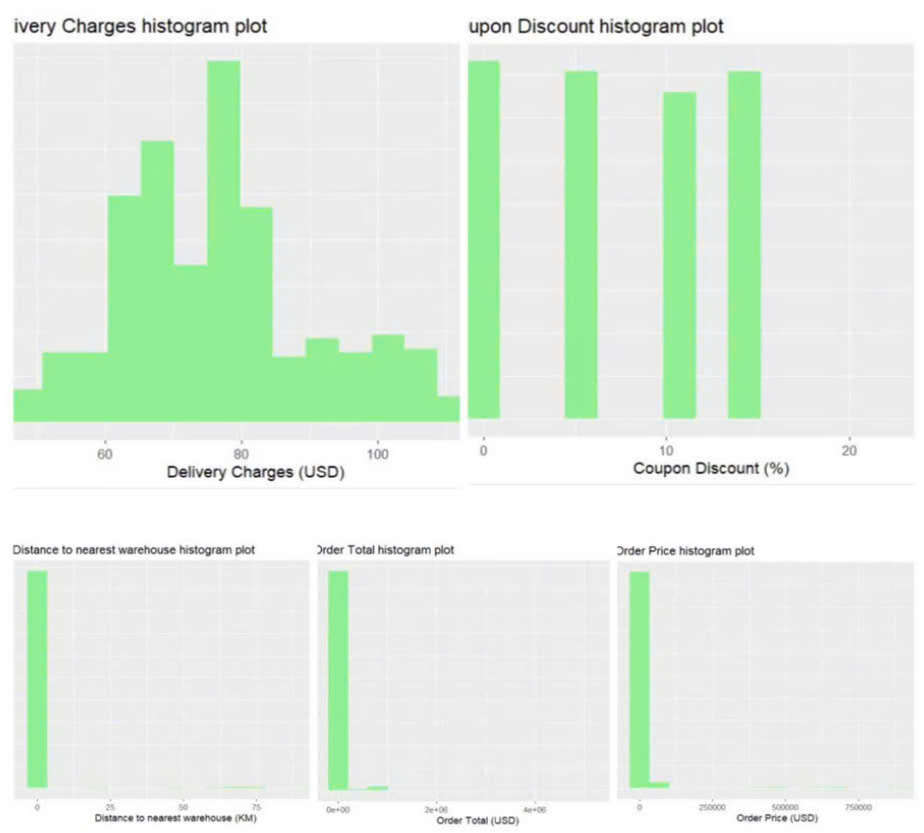
\includegraphics[width=0.7\linewidth]{graphics/bang7.jpg}
    \caption{Đồ thị Histogram của các biến liên tục}
  
\end{figure}
* Nhận xét: Ta nhận thấy rằng, từ kết quả đồ thị histogram cho thấy biến order\_total, order\_price, distance\_to\_nearest\_warehouse có phân phối lệch phải, với một cột cao ở phía bên trái. Điều này cho thấy hầu hết khách hàng chỉ chi tiêu ở mức thấp hơn, trong khi một số ít có tổng giá trị đơn hang cao, tạo ra các điểm ngoại lệ. Phân phối lệch phải thường cho thấy  rằng có một số khách hang chi tiêu rất cao, điều này có thể ảnh hưởng đến quy mô hình hồi quy. Sau khi kiểm tra tỉ lệ khuyết nhỏ của các ngoại lai .Để xử lí tình trạng phân phối lệch phải này.\\
 -->Ta áp dụng xóa bỏ các ngoại lai  của order\_total, order\_price, distance\_to\_nearest\_warehouse.\\
 Dưới đây là hình ảnh sau khi xóa ngoại lai.
 \begin{figure}[H]
    \centering
    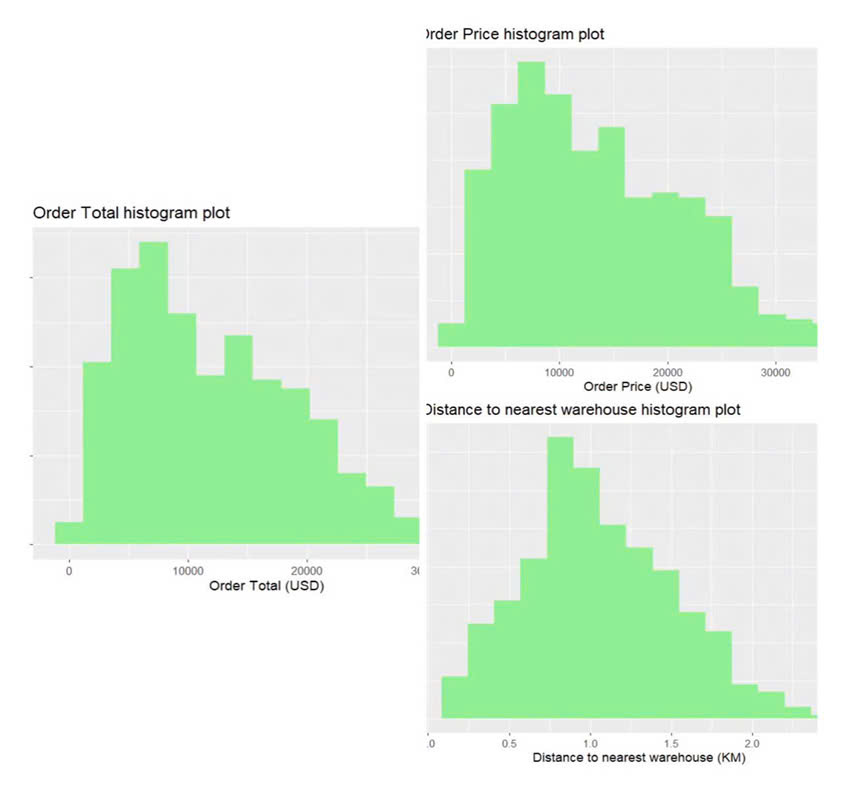
\includegraphics[width=0.7\linewidth]{graphics/bang8.jpg}
    \caption{Đồ thị Histogram của các biến liên tục đã xóa ngoại lai}
    
\end{figure}
\subsection*{\subsection*{4.2.2 Đồ thị phân tần}}
Ta so sánh  lần lượt từng order\_price, delivery\_charges, coupon\_discount, distance\_to\_nearest\_warehouse với order\_total.
\begin{figure}[H]
    \centering
    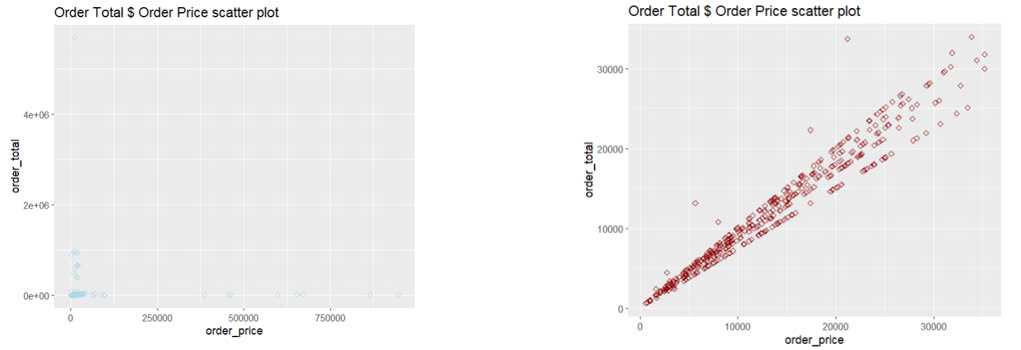
\includegraphics[width=0.8\linewidth]{graphics/bang9.jpg}
    \caption{Hình chưa xóa ngoại lai và đã xóa của order\_price}
 
\end{figure}
\begin{figure}[H]
    \centering
    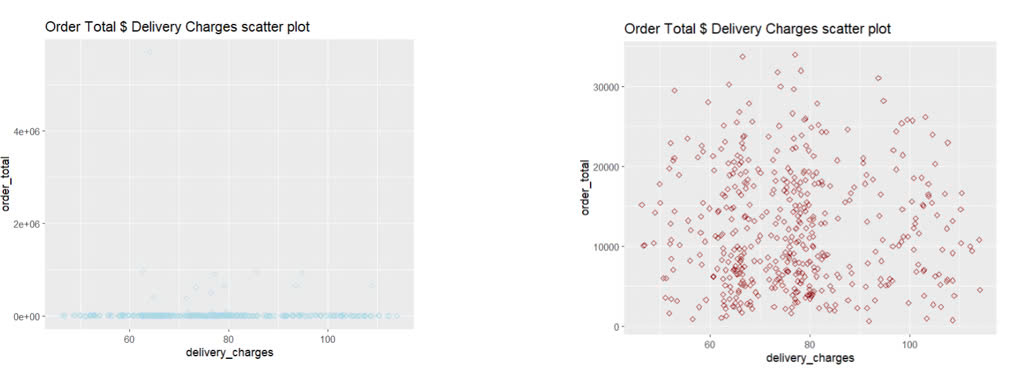
\includegraphics[width=0.8\linewidth]{graphics/bang10.jpg}
    \caption{Hình chưa xóa ngoại lai và đã xóa của delivery\_charges}
    
\end{figure}
\begin{figure}[H]
    \centering
    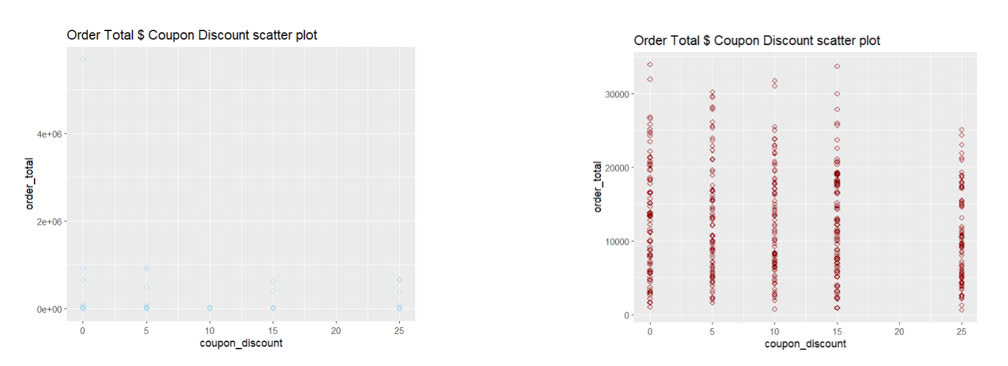
\includegraphics[width=0.8\linewidth]{graphics/bang11.jpg}
    \caption{Hình chưa xóa ngoại lai và đã xóa của coupon\_discount}
    
\end{figure}
\begin{figure}[H]
    \centering
    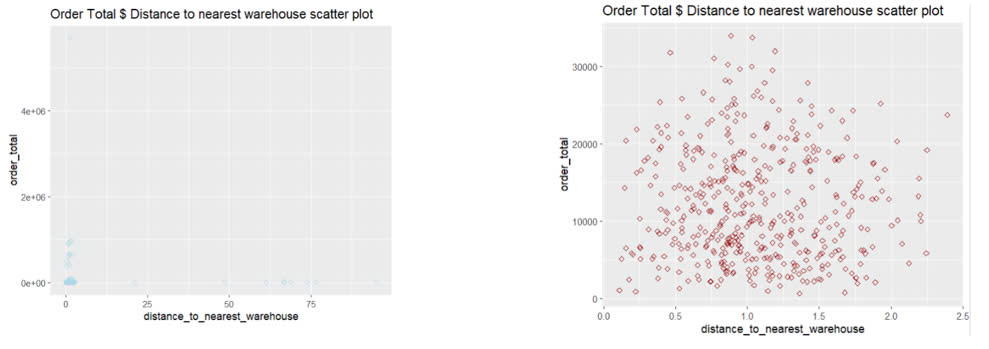
\includegraphics[width=0.8\linewidth]{graphics/bang12.jpg}
    \caption{Hình chưa xóa ngoại lai và đã xóa của distance\_to\_nearest\_warehouse}
 
\end{figure}
Với những hình ảnh có những chấm màu xanh là chưa xóa ngoại lai, còn những hình có chấm màu đỏ là đã xóa ngoại lai. \\
*Nhận xét: \\
•	Hai biến order\_price và coupon\_discount là 2 biến có ảnh hưởng tới order\_total hay còn gọi là có quan hệ tuyến tính.\\
•	Hai biến delivery\_charges và distance\_to\_nearest\_warehouse không có ảnh hưởng tới order\_total hay không có quan hệ tuyến tính.
\subsection*{\subsection*{4.3 Phân tích biến định lượng bằng biểu đồ boxplot }}
Ta phân tích biến order\_total theo các biến nearest\_warehouse, season, is\_expedited\_delivery, is\_happy\_customer.
\begin{figure}[H]
    \centering
    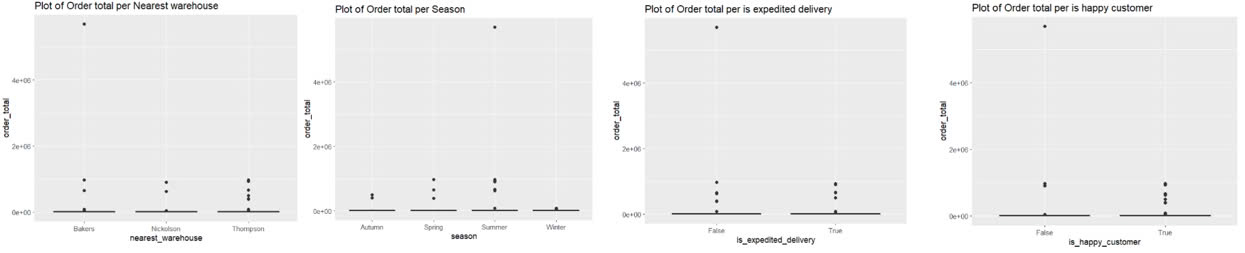
\includegraphics[width=1\linewidth]{graphics/bang13.jpg}
    \caption{Biểu đồ boxplot chưa xóa ngoại lai của các biến định lượng}
    
\end{figure}
\begin{figure}[H]
    \centering
    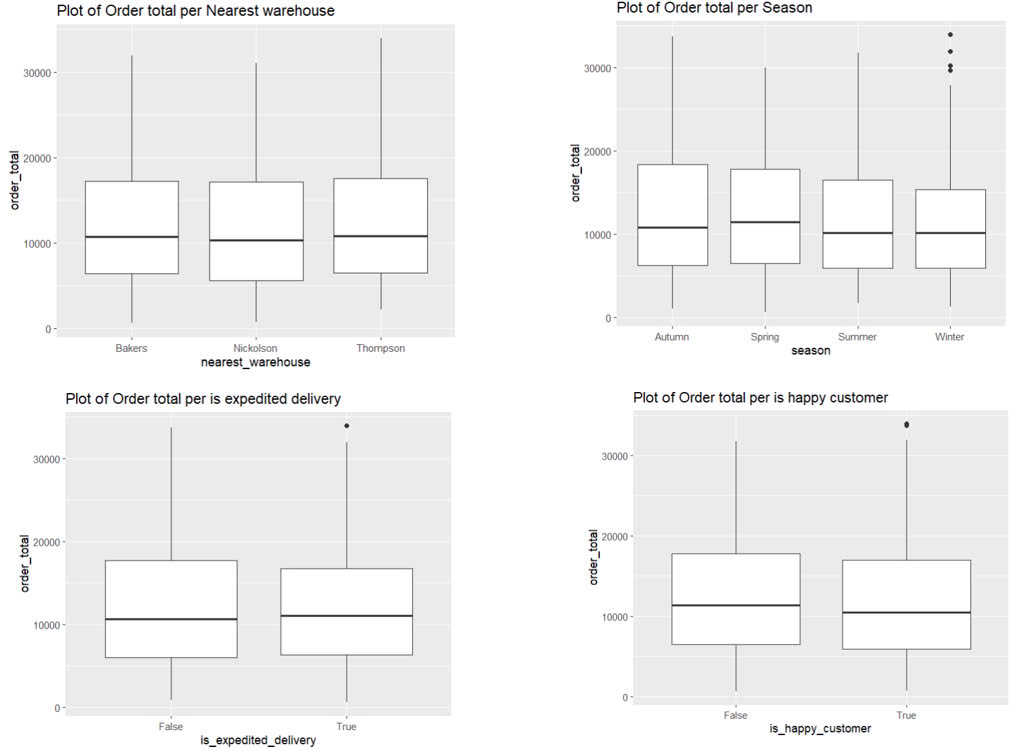
\includegraphics[width=1\linewidth]{graphics/bang14.jpg}
    \caption{Biểu đồ boxplot đã xóa ngoại lai của các biến định lượng}
    
\end{figure}
*Nhận xét: lần lượt cho  nearest\_warehouse, season, is\_expedited\_delivery, is\_happy\_customer.\\
•	Cả ba kho hàng (Bakers, Nickolson, Thompson) đều có phân bố tổng đơn hàng tương tự nhau, với các giá trị trung vị (median) gần như ngang bằng.\\
•	Phân bố giá trị order\_total khá đồng đều qua các mùa, tuy nhiên mùa Đông có một vài đơn hàng nổi bật với giá trị rất lớn.\\
•	Hình thức giao hàng nhanh dường như không có ảnh hưởng rõ rệt đến tổng giá trị đơn hàng trong phần lớn các trường hợp.\\
•	Trạng thái hài lòng của khách hàng không tạo ra sự khác biệt lớn trong tổng giá trị đơn hàng, nhưng nhóm khách hàng hài lòng có xu hướng chi tiêu nhiều hơn một chút và có thể thực hiện các đơn hàng có giá trị rất lớn (outliers).
